\pagenumbering{arabic}

\chapter{Introduction} \label{introduction}

For further explanation and details, please, turn to the referred clauses of IEEE 29148-2018, the highlighted and commented version; pay attention to the comments. Clause numbers are written in \textit{italic} in the sections.

Refer to \textit{(Clause 9.6.1)}. 

\section{Purpose of the System }

The purpose of the FarmBot system is to revolutionize agricultural practices through automation. FarmBot aims to regularize farming methods, enhance crop yields and minimize resource waste. Additionally; FarmBot provide a platform to manage and monitor their crops and agricultural operations efficiently. Through automation and monitoring, the system aims to:

\begin{itemize}
    \item Automate planting, watering, weeding and harvesting processes to reduce human work and improve efficiency.
    \item Provide precise control over the environmental factors such as soil moisture, harmful weeds.
    \item Facilitate real-time monitoring from web application to enhance crop health.
    \item Provide an environment to design a layout for crops and implement that design in real world.
\end{itemize}

\section{Scope}

Refer to \textit{(Clause 9.6.3, 9.5.3, 9.4.3)}

\section{System Overview}


\subsection{System Perspective}

\begin{figure}
  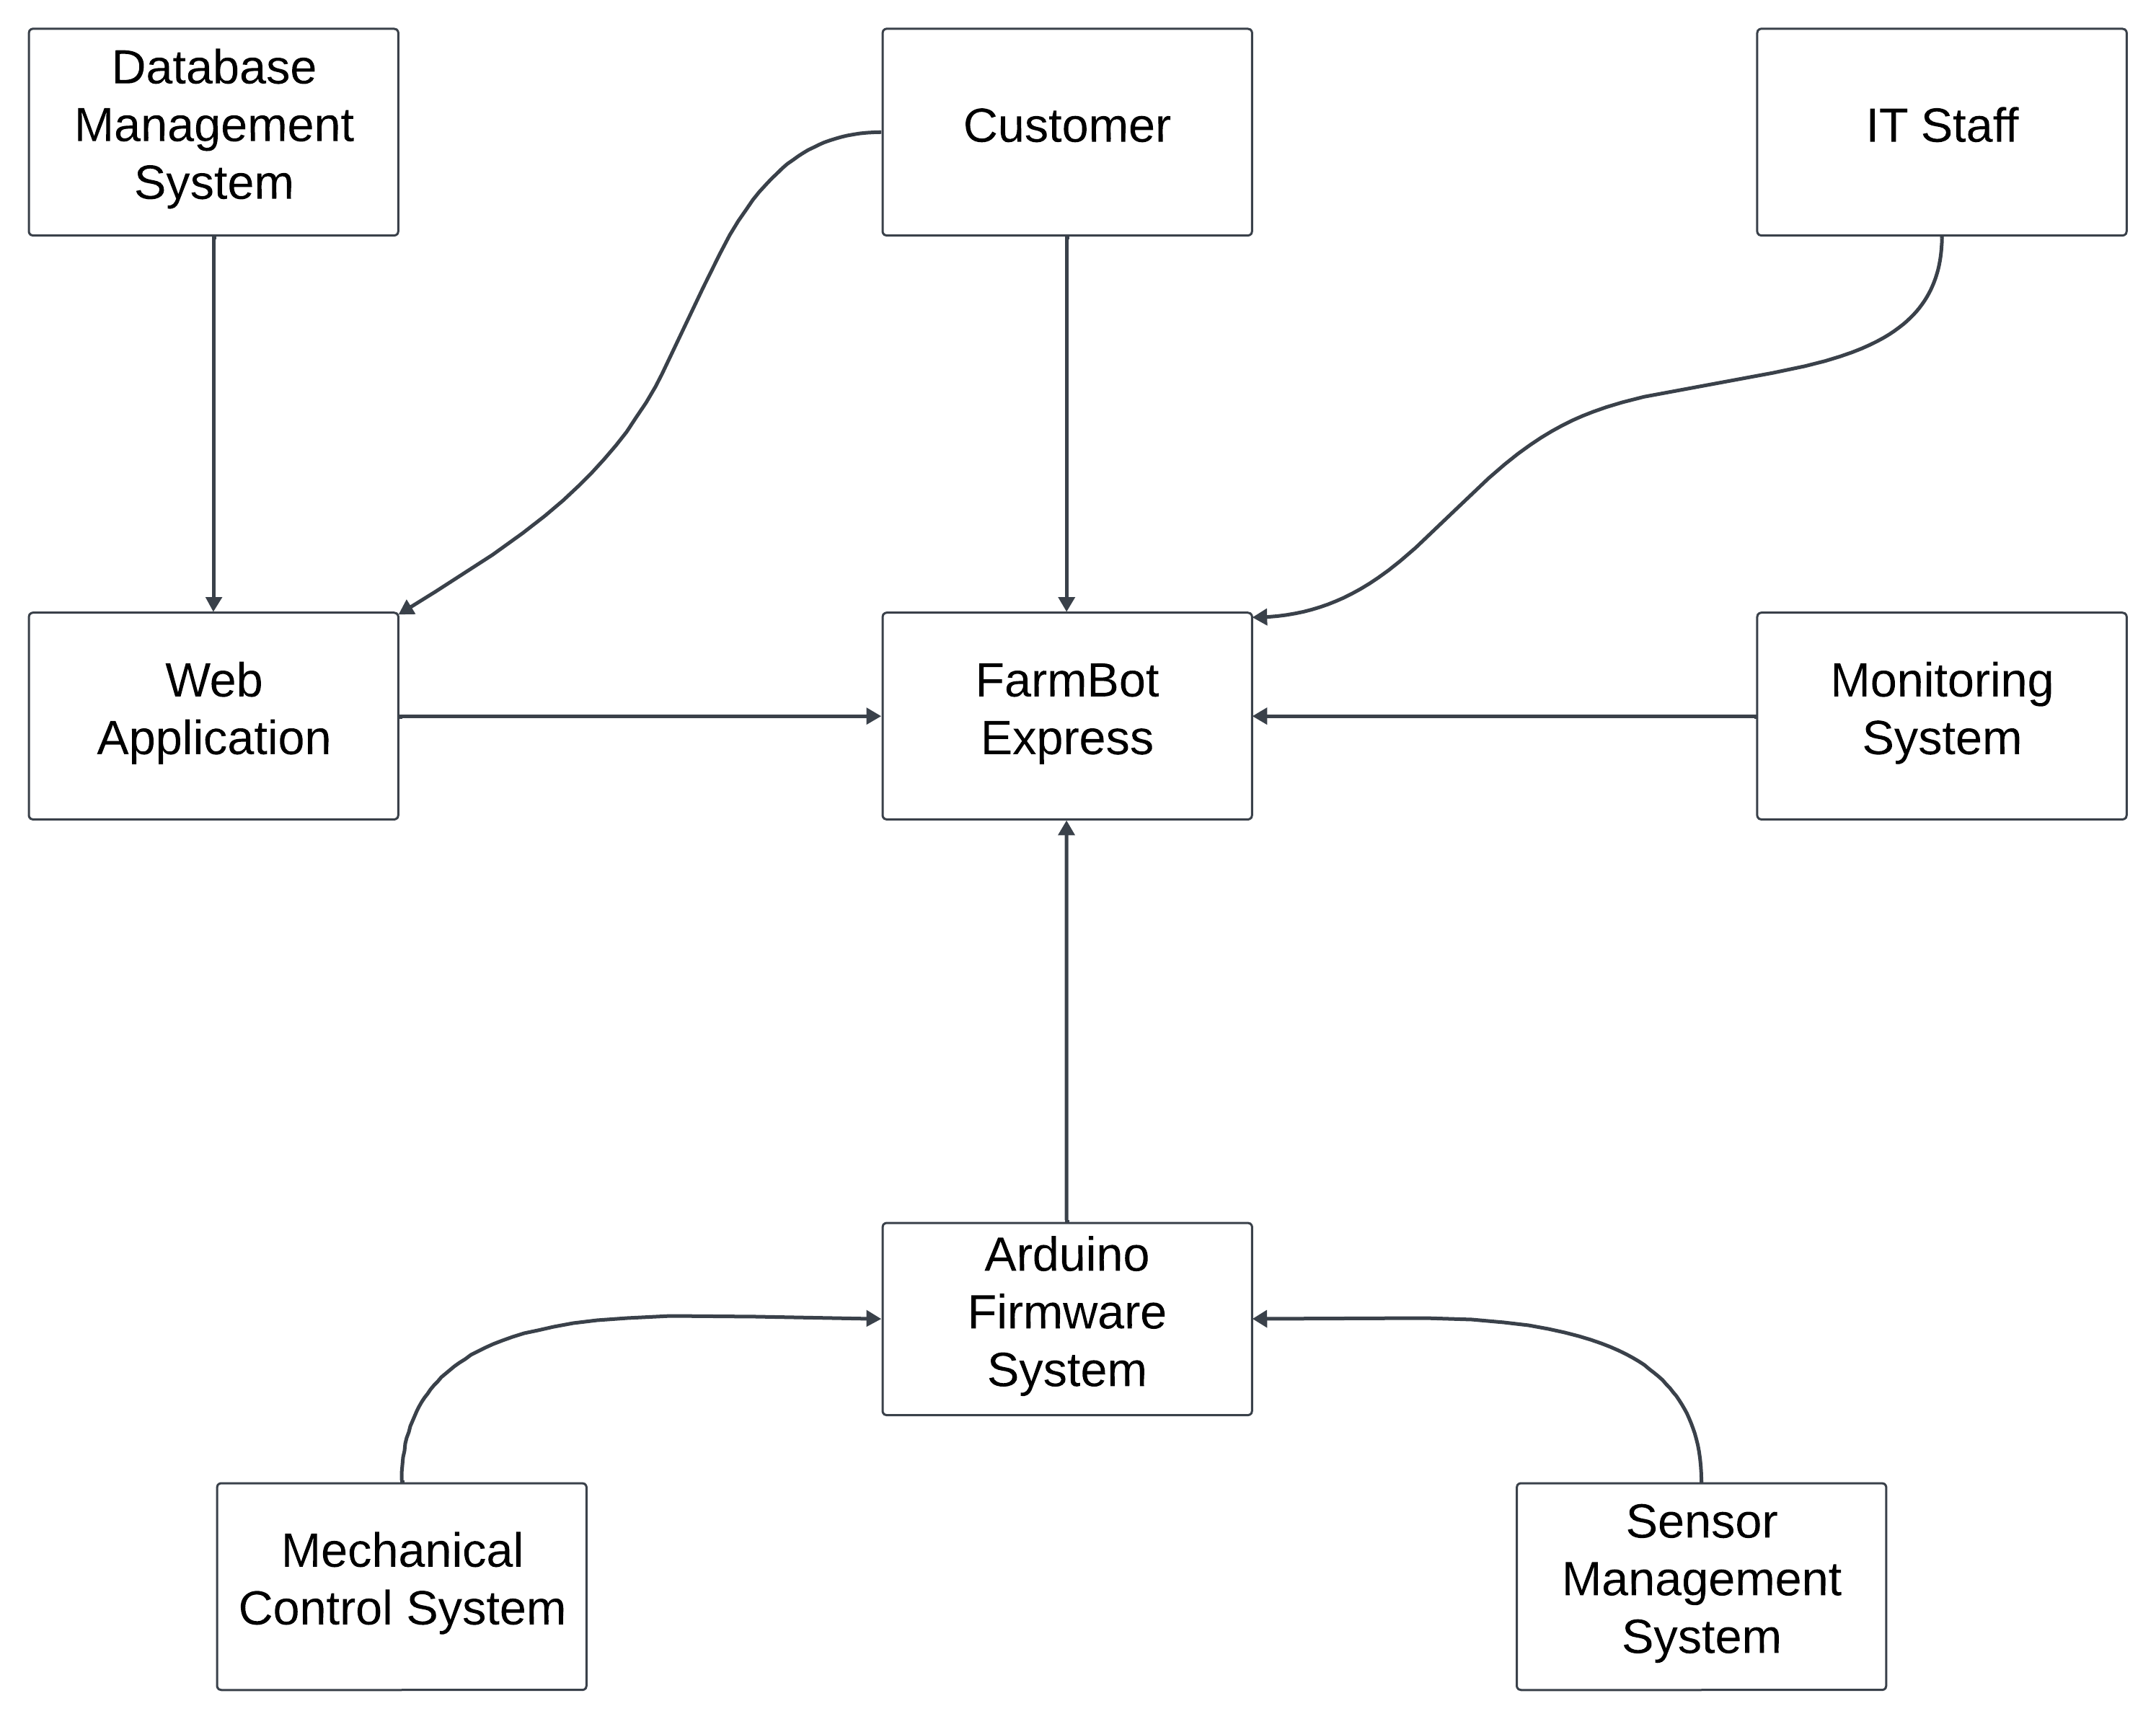
\includegraphics[width=\linewidth]{Figures/context-diagram.png}
  \caption{Context Diagram of FarmBot Express}
\end{figure}

Refer to \textit{(Clause 9.6.4, 9.5.4.1)}
\subsubsection{System Interfaces}
Refer to \textit{(Clause 9.6.4.1)}
\subsubsection{User Interfaces}
Refer to \textit{(Clause 9.6.4.2)}
\subsubsection{Hardware Interfaces}
Refer to \textit{(Clause 9.6.4.3)}
\subsubsection{Software Interfaces}
Refer to \textit{(Clause 9.6.4.4)}
\subsubsection{Communication Interfaces}
Refer to \textit{(Clause 9.6.4.5)}
\subsubsection{Memory Constraints}
Refer to \textit{(Clause 9.6.4.6)}
\subsubsection{Operations}
Refer to \textit{(Clause 9.6.4.7)}

\subsection{System Functions}

Refer to \textit{(Clause 9.6.5, 9.5.4.2)}. If you want to add any figure or diagram, you can use a figure environment.In Figure \ref{Fig:Example}

\begin{figure}[ht]
\centering
\includegraphics[width=.9 \textwidth]{Figures/ExampleFigure.png}
\caption{Example \label{Fig:Example}}
\end{figure}


\subsection{Stakeholder Characteristics}

Refer to \textit{(Clause 9.6.6, 9.5.4.3, 9.4.5)}

\subsection{Limitations}

Refer to \textit{(Clause 9.6.7)}

\section{Definitions}

You should add acronyms and abbreviations here. Refer to \textit{(Clause 9.6.7)}



For any citation, refer to it as \cite{younis2021hybrid}.
